\chapter{\protect Astrophysical Implications}
\label{astron}

The main source to irradiating the dark side of Charon is Ly$\alpha$, reflected by interplanetary medium \cite{grundy2016formation}. Other sources include energetic ions in solar wind, which mainly consist of H$^+$, He$^+$, He$^{++}$ and O$^{2+}$ ,etc. originated from solar corona or IPM. Helium ion emits He II line in all directions when they falls back to the ground state including the dark side of Charon. He II irradiation as it is 3 to 20 times more intense than He I during a solar flare. As the intensity varies with solar activities, it is difficult to estimate the dose onto Charon.

In this chapter, we will discuss the impacts of three difference energy sources , including EUV, VUV and energetic (5 keV) electrons on production of cyanide ions and their implication on Charon. First, we compare the destructive cross-sections of these sources, and then their corresponding production yields in CN$^-$.

\section{The destruction of methane and ammonia by photon sources and electrons}

In electron irradiation experiments of Kim and Kaiser (2011)\cite{kim}, the energy transferred to CH$_4$ + NH$_3$ ice mixtures is by linear electron transfer (LET) of 3.1 keV $\mu$m$^{-1}$, in the order of magnitude of the MeV cosmic rays typically transferred to the ice samples. Their dose reached 1.3 eV molecule$^{-1}$ in 90 minutes with about 610 ML of CH$_4$ and 260 ML of NH$_3$. 

The percentage of photons absorbed by CH$_4$ and NH$_3$ ice mixtures under VUV irradiation is calculated by substituting cross-sections measured by Cruz-Diaz et al. (2014) \cite{cruz2014vacuum} and the VUV intensity spectrum of our MDHL into Beer$'$s law. CH$_4$:NH$_3$ = 3:2 ice mixtures can absorb more than 99 \% of light when thickness of NH$_3$ equals 600 ML (figure \ref{fig:absorption_percentage}). Therefore, we may assume all the irradiated light is absorbed by the ice. For CH$_4$:NH$_3$ =3:2 ice mixture, around 9 $\times$ 10$^{17}$ photons are irradiated in 270 minutes.

Regarding EUV irradiations, since there are no suitable windows (used for cutting off higher order lights) to measure the absorption of ices, it is impossible to obtain absorption cross-sections right now. From figure \ref{fig:normalized_reactants}, we obtain the distructive cross-sections of EUV to VUV photons. The CH$_4$ destruction by EUV photons is 6.06$\pm$0.07 times lower than VUV irradiation.  From the New Horizons Mission, EUV irradiation (>12.4 eV) is $8.7 \times 10^7 eV cm^{-2} s^{-1}$ at mean heliocentric distance (39 A.U.) of Charon whereas VUV irradiation (Ly-$\alpha$ photons) is 1.9 $\times$ 10$^9$ eV cm$^{-2}$ s$^{-1}$\cite{grundy2016formation}. Since VUV flux is one order of magnitude more intense then EUV fluxes and the CH$_4$ destruction is about 6 times higher than EUV irradiation, it is the main source causing the destruction of CH$_4$.

\begin{figure}
\centering
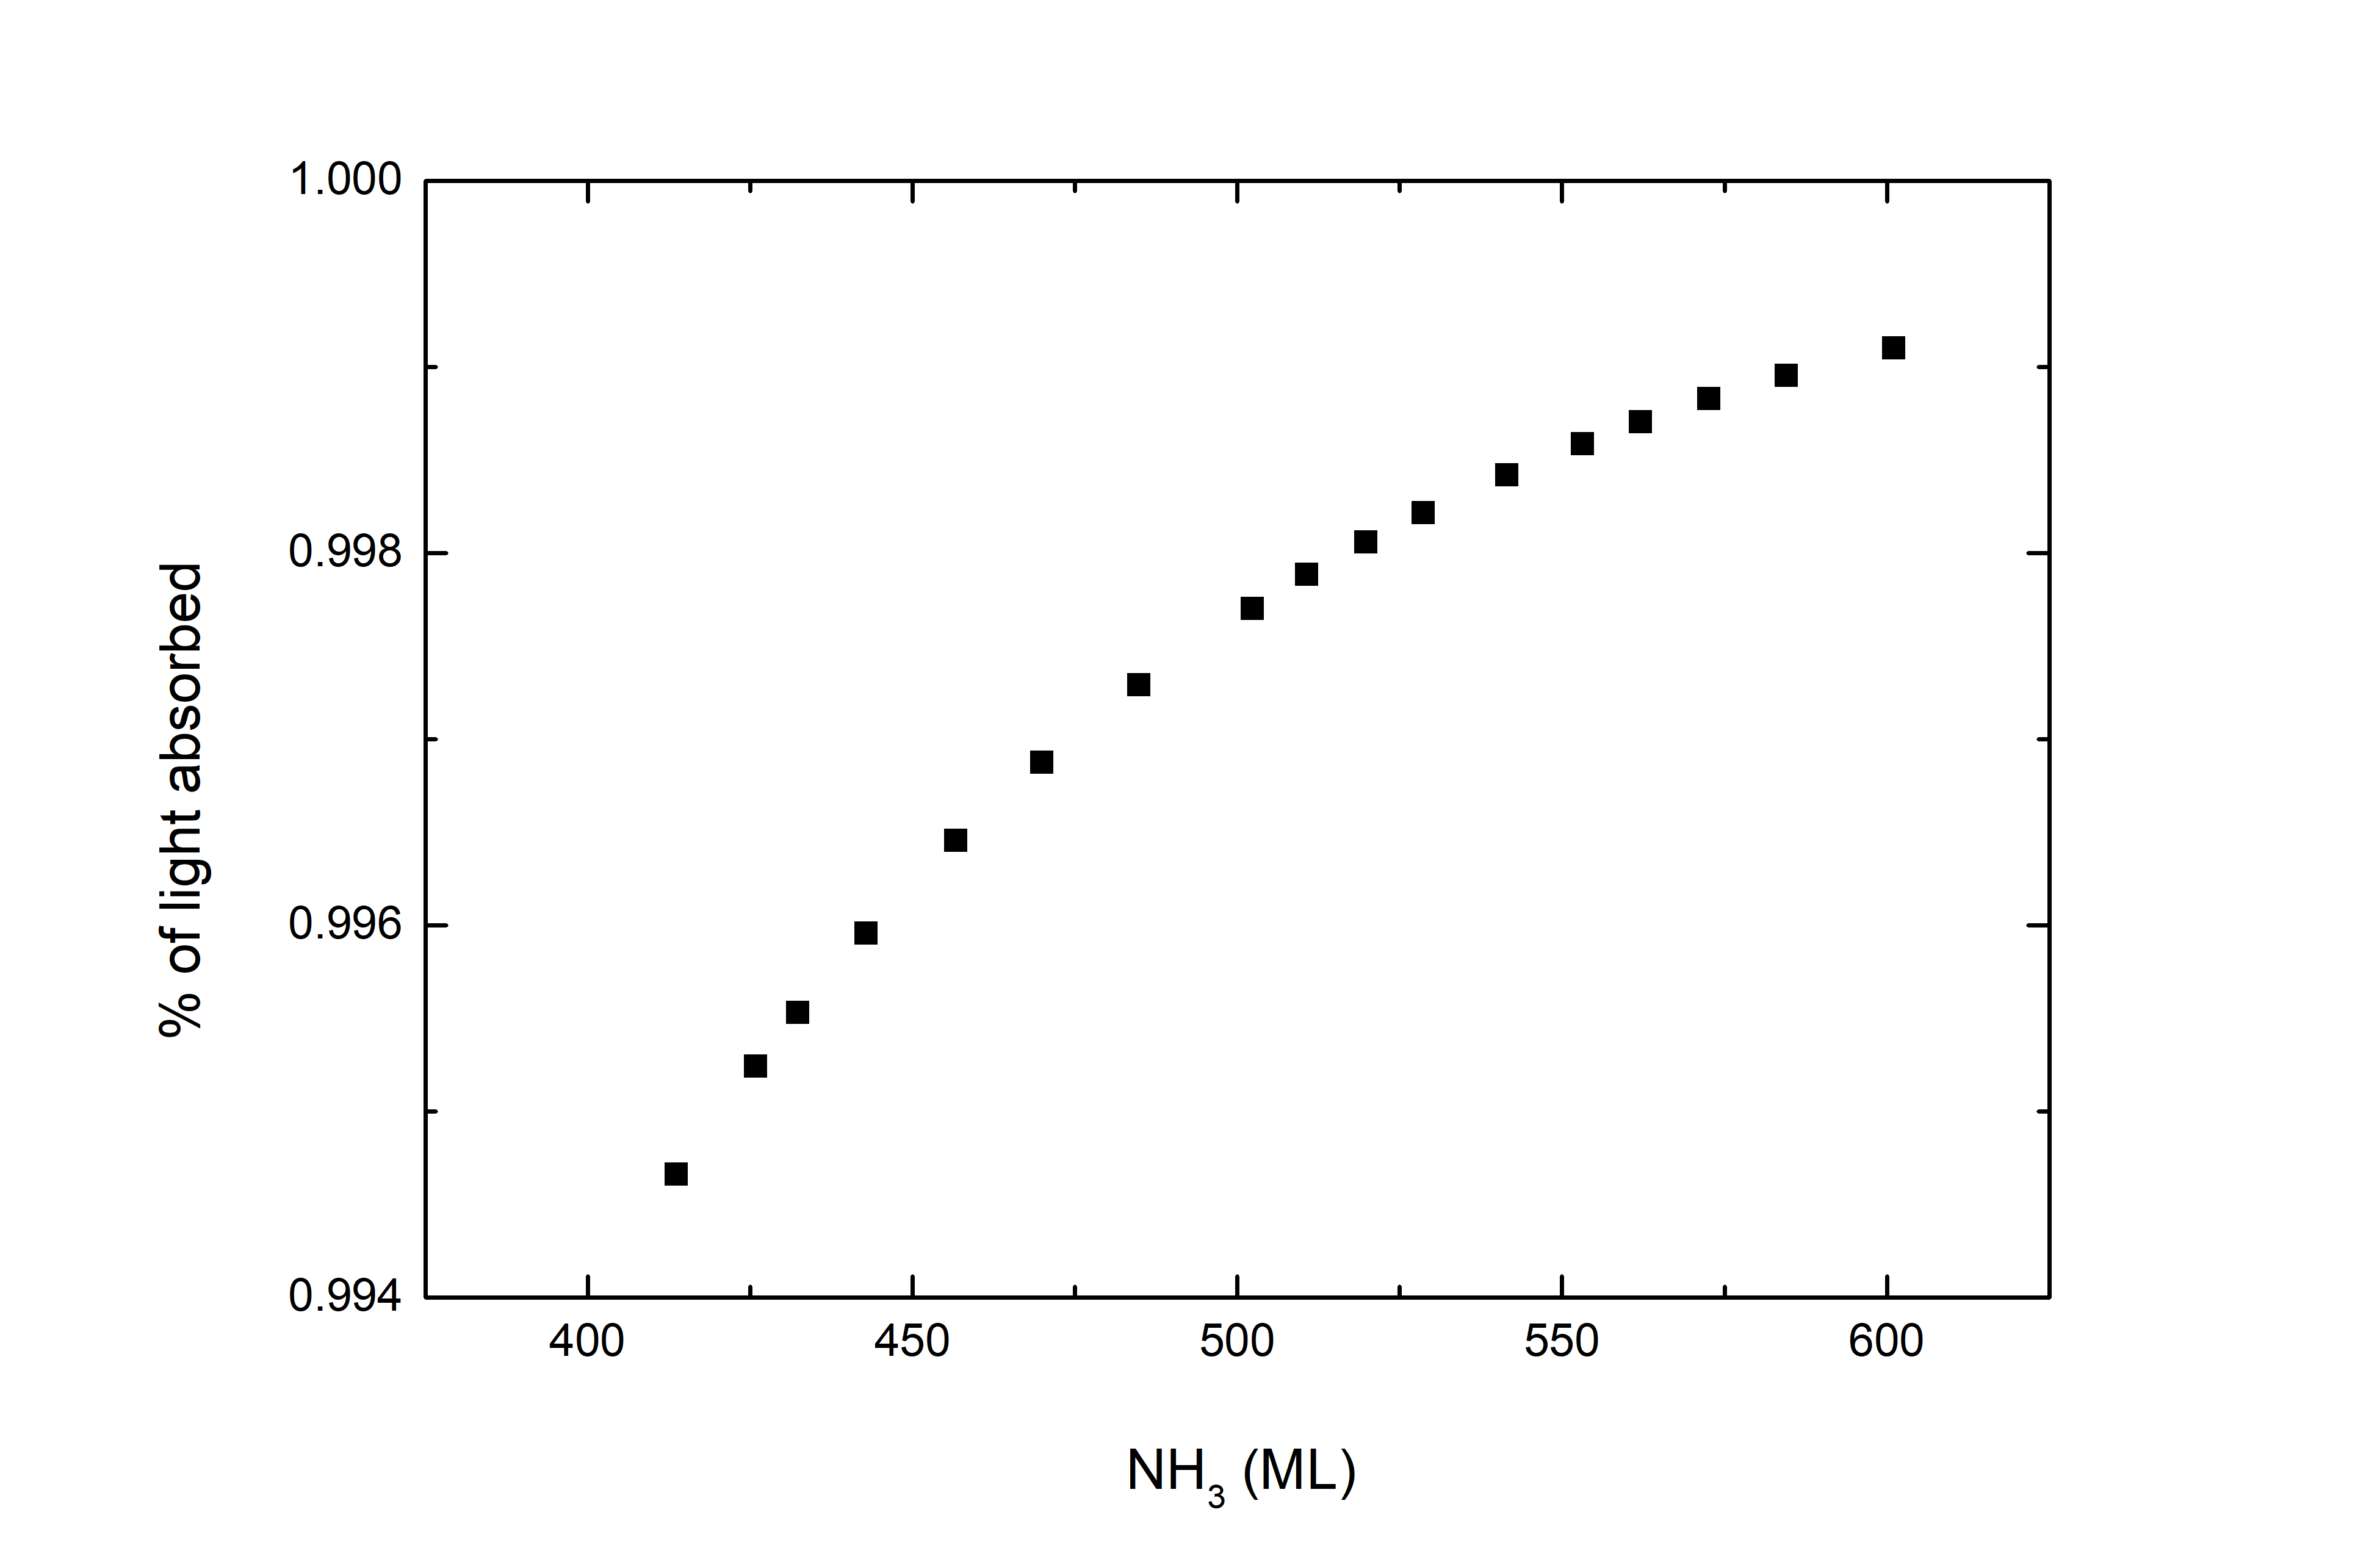
\includegraphics[width=\textwidth]{figures/chapter4/absorption_percentage.png}
\caption{The calculated percentage of VUV irradiation absorbed by different thickness of CH$_4$ to NH$_3$ = 3:2 ice mixtures.}
\label{fig:absorption_percentage}
\end{figure}

\section{Cyanide ion produced by photon sources and electrons} %comparison with Kim use beer's law to get the total irradiated ice 

Considering the ice mixtures in which CH$_4$ is dominated, the efficiencies in CN$^-$ formation by electrons and VUV irradiations is calculated by the final column densities divided by the column densities of the limiting reactant. A fixed amount of CN$^-$ is obtained after irradiations. In our MDHL experiments, we have 14.8 ML of CN$^-$ obtained in (CH$_4$ = 900 ML, NH$_3$= 600 ML) ice mixtures. Kim and Kaiser (2011) irradiated  ice mixtures(CH$_4$ = 610 ML, NH$_3$= 260 ML) and obtained 13 - 16 ML of CN$^-$ adopting the CN$^-$ absorption coefficient (3.7 $\times$ 10$^{-18}$ cm molecule$^{-1}$) \cite{georgieva2006computational}, which is 4.86 times smaller than the absorption strength adopted. We do not adopt the same absorption coefficient because the absorption strength is based on gas phase experiments and models. We adopted the absorption strength calculated by Noble et al. (2012) \cite{noble2012thermal} based on experiments mixing CH$_4$ and NH$_3$ in room temperatures and deposited at 20 K. If they adopt the same absorption coefficient, the production yield of CN$^-$ should be divided by 4.86. Therefore, regarding percentage of NH$_3$ (limiting reactant), Kim and Kaiser has 1 \% yield where we have 2.47 \% yield in relative proportion of CH$_4$:NH$_3$ = 3:2.

The depositing rates of CH$_4$ onto the surface of Charon, varies by the surface area below 25 K (see chapter \ref{introduction} for details). The arrival flux is 2 $\times$ 10$^{24}$ s$^{-1}$ \cite{hoey201}. From calculation of Grundy et al. (2016), CH$_4$ do not acquire sufficient energy to escape Charon and after 7 hops, it arrive the surfaces below 25 K. In 1 pluto winter (130 earth years), around 173 ML of CH$_4$ will be deposited onto the poles. Since Charon-pluto is a tidal locked relation, it is resonable to predict that one of the surface is with more CH$_4$ hitting rates and hence condenses more CH$_4$.

The experimental situation is ideal to apply on very thick ices, where photons or electrons can irradiate the surface without renewal since(covered by non-irradiated CH$_4$ ice) we have nearly 100 percent absorption in VUV photons(figure \ref{fig:absorption_percentage}). Our experimental results can be applied to calculate the surface column densities of CN$^-$ and C$_2$H$_6$ on Charon after the winter times. The ice would be further processed by EUV or other energetic energy sources when directly facing to the sun. Therefore, information of pre-irradiated ices during winter times is helpful to future studies, of which compositions are known for irradiation experiments by other energetic sources like electrons.\\

From our experiments, irradiation of 7.6 $\times$ 10 $^{17}$ VUV photons is the irradiations irradiated on Charon in about 0.5 Pluto year. As a result, under winter time, if we only consider VUV photon source, assuming ratio of CH$_4$ to NH$_3$ is 3:2, 1:5, 1:10 and 1:20, about 22.5, 36.6, 29.5 and 18.9 ML of CN$^-$ will be formed during winter time respectively(figure \ref{fig:CN_NSRRC}).

\section{Conclusion}
Through investigating methane(CH$_4$) and ammonia(NH$_3$) ice mixtures, we better understand the followings relations: 1. The formation yield of cyanide ion (CN$^-$) is not proportional to the initial deposited methane when methane is dominating. However, the formation rate is proportional to its initial CH$_4$ to NH$_3$ ratios. The competition between CH$_3$ radicals (forming both CH$_3$NH$_2$ and C$_2$H$_6$) and NH$_2$ radicals (forming CH$_3$NH$_2$) results in the former result. 2. When VUV is replaced by 40.8 eV 30.4nm (40.8 eV) He II EUV irradiations, the destruction cross-section of CH$_4$ and NH$_3$ are reduced by  6.06$\pm$0.07 and 3.19$\pm$0.12 times respectively. The lower formation rate of CN$^-$ in EUV irradiation by 3.06 to 4.13 times is mainly due to the reduced NH$_3$ destruction cross-sections. 3. The functional groups of residues obtained in CH$_4$ to NH$_3$ = 3:2 ice mixtures are similar to the laboratory made Titan tholins. 4. The formation of CN$^-$ with different ratios of CH$_4$ to NH$_3$ ice mixtures provides valuable informations on the surface compositions of Charon after winter time.

